\chapter{Thesis Conclusion}

\begin{flushright} 
\textit{"Begin at the beginning and go on till you come to the end: then stop."
\\-Lewis Carroll, Alice's Adventures in Wonderland.}\end{flushright} 
\begingroup
  %\vspace*{\beforechapskip}%
  %\smash{\rule{2.6pt}{25mm}} 
\textit{This chapter recapitulates and highlights the main contributions of this thesis and sets them again in relation to each other, relating them to the
 overarching theme of more robust context recognition. Moreover, we discuss
 the limitations of this work giving guidance for improvements. We end with a
 perspective and future research directions implied by the work
 presented.} \\\\\\ Kunze, K., Bahle, G., Lukowicz, P., and Partridge,
 K. Can magnetic field sensors replace gyroscopes in wearable sensing
 applications \textit{In Proceedings of the 2010 11th IEEE ISWC}. Seoul, South Korea,
 2010.\\
 Kunze, K., Lukowicz, P. Combining Crowd-based Sensing, Microblogging and Activity Flow Models: A case study using soccer games
 \textit{Workshop on Hybrid Pervasive/Digital Inference (HPDI 2011) }. San Francisco, USA, 2010.
 \vskip\onelineskip
\vskip\onelineskip
\begin{adjustwidth}{}{-\chapindent}%
\hrulefill  
\end{adjustwidth}\endgroup
\vskip\onelineskip
\vskip\onelineskip 
This thesis investigated on-body placement effects in context recognition.
Although the topic is very relevant in regards to building real-life pervasive applications,
it gains special importance in the light of a recent trend in pervasive research,
the use of commodity appliances (e.g. smart phones) for context recognition.
The most important contributions of this thesis towards more real-life
context-aware applications are, in my opinion, the active sampling
approach using audio to infer symbolic location in Chapter 2, the
on-body placement detection in Chapter 3 and the heuristics presented
to deal with displacement in Chapter 4.
In the following, we discuss the contributions, go over potential limitations and
the relevance of this thesis to the research field.
Finally, in the outlook some future work directions are given.

\section{Contributions Overview}

\begin{figure}[t]
  \begin{center}
  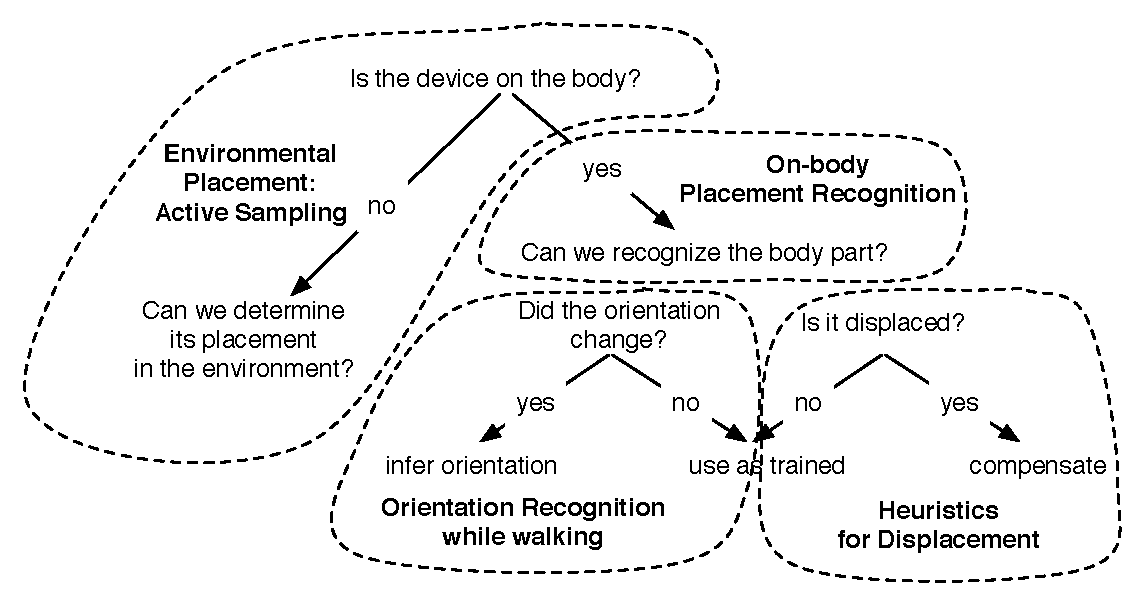
\includegraphics[height=2.3in]{ConclusionOverview.pdf}
	\end{center}
  \caption[Thesis contributions]{Thesis Overview with core contributions highlighted}
\label{fig:ConclusionGraph}
\end{figure} 
Problems related to on-body sensor placement are essential for pervasive computing, especially with the proliferation of smart appliances. This thesis provides some major advances understanding and tackling these problems. Subsequently, we put the thesis in relation with the aims section~\ref{aims} presented in the motivation. 
\begin{enumerate}
\item I present a categorization of different placement factors (as seen in Figure~\ref{fig:ConclusionGraph}). I discuss the effects of the placement factors on common sensing modalities using signal examples, conceptional analysis and quantitative evaluations, where possible. The focus of my work is on motion sensors, especially accelerometers, as they are very common in on-body context sensing. Still, most placement effect discussions also include sound, radio signal strength, gps, gyroscopes and magnetic field sensors.
\item Techniques and approaches are presented that reduce the particular placement effects for a given sensing modality (e.g. low pass filtering, displacement robust features).
\item Finally, I develop methods to infer the environmental symbolic location, the on-body placement and the orientation of a device. In addition, I give heuristics to deal with displacement in motion based inference. The methods are all very general, working for a wide range of scenarios and validated using extensive experimental evaluation. The application scenarios range from house work over sport exercise to machine repair. The users vary significantly in age (from 21 to over 60) and profession. The experimental recordings include in total over 60 hours of multimodal sensor data. A lot of the data sets are either publicly available or shared with a smaller circle of researchers in the field.
\end{enumerate}

There three types of device placement variations were introduced: coarse variations, fine grain
variations and variations directly related to orientation. These
types of variations directly relate to the main research problems
dealt with in this thesis, shown in Figure~\ref{fig:ConclusionGraph}.

\begin{description}
\item{Environmental Placement} -- The questions "Is the device on the body?", "Can we determine its
placement in the environment" are tackled in Chapter 2. The thesis contribution towards solving
these questions is an environmental placement detection using active sampling. 
This active sampling approach requires only simple sensors (acceleration,
sound) and no infrastructure setup. The method works for specific
placements such as 'on the couch', 'in the desk drawer' as well as for
general location classes, such as 'closed wood compartment' or 'open
iron surface'. In the experimental evaluation we could reach a
recognition accuracy of 90 \% and above over a total of over 1200 measurements from 35
 specific locations (taken from 3 different rooms) and 12 abstract
 location classes. 
\item{On-body Placement} -- The on-body placement recognition derives the coarse
device placement solely based on rotation and acceleration signals
from the device. It works regardless of device orientation.
 The on-body placement recognition rate is around 80 \%
 over 4 min. of unconstrained motion data for the worst scenario and
 up to 90 \% over a 2 min. interval for the best scenario.
We use over 20 hours of motion data for the analysis.
\item{Displacement} -- "Is it displaced?" deals with variations related
to displacement and is handled in Chapter 4, where clear displacement
heuristics are presented for inertial motion sensors. 
Our heuristic raises the displaced recognition rate
from 24\% for a displaced accelerometer, which had 96\% recognition
 when not displaced, to 82\%. 
\item{Orientation} -- "Did the orientation change?", in turn, then relates to variations due to
altering the device orientation. Chapter 5 presents a method to infer
the device orientation while the user is walking based solely on
acceleration.
\end{description}

Pervasive computing applications that utilize my findings to cope with device placement issues have major advantages: 
\begin{description}
\item{Resilience} -- The introduced methods enable motion based context recognition systems to function despite
sensor placement changes. The methods work with dedicated wearable systems as well as with novel sensing approaches using smart appliances.
\item{Novel context recognition methods} -- The techniques discussed are meant to support motion based context recognition systems to make their inference more robust. Additionally, most techniques can be used directly as a source for contextual information. The fact that a device is placed at a symbolic location or on a specific body part gives already some clues about the user's current situation.
\item{Higher user acceptance and better usability} -- Especially when using sensors equipped in smart appliances, the user cannot be expected to fix sensors to narrowly defined on-body placements. Some of the solutions shown here have been already successfully applied to phone based sensing in various applications, from gym exercise to assisted living~\cite{Muehlbauer:2011ir,Bahle:2010ww,Franke:2009ei}. The findings of this thesis are relevant to a wide range of application scenarios. The user has to bother less about the placements of his devices and can focus more on the task at hand. This makes already existing pervasive applications more acceptable to the user and enables new use cases for motion based inference.
\end{description}

Overall, I present a well balanced overview of placement effects in context recognition,
categorized them as given in Figure~\ref{fig:ConclusionGraph} and provided for each category 
a solution approach for motion based inference. 

\section{Limitations and Relevance}

\begin{figure}[t]
  \begin{center}
  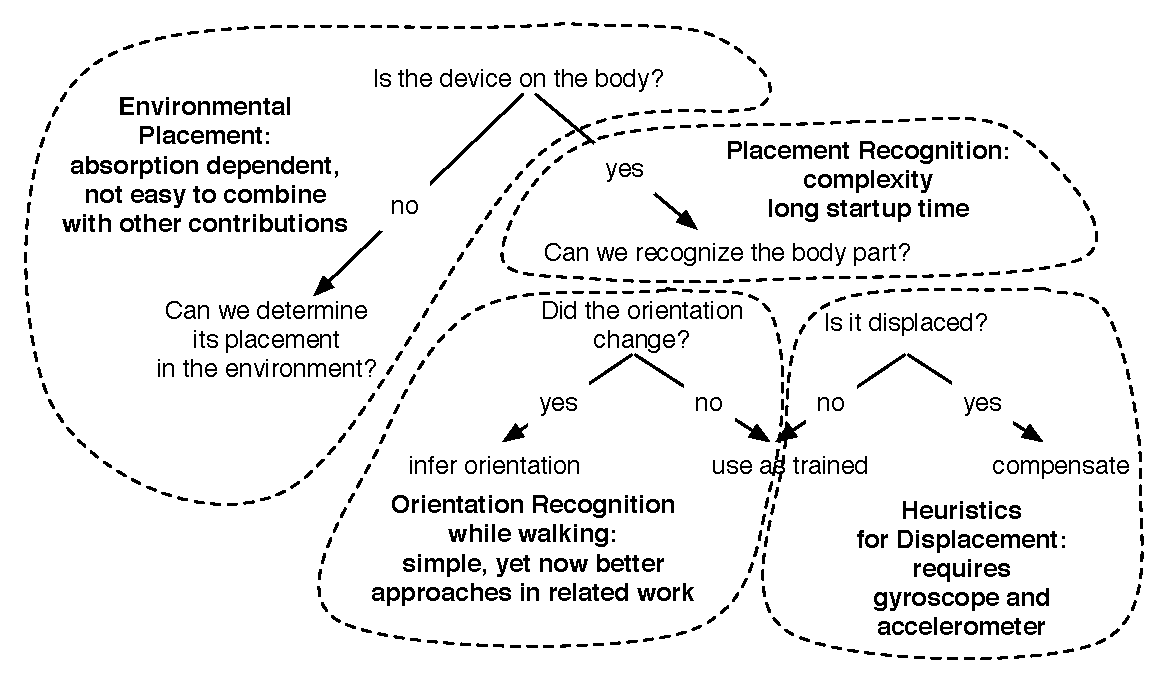
\includegraphics[height=2.3in]{limitations.pdf}
	\end{center}
  \caption[Thesis limitations]{The limitations of this thesis related to the sub-topics.}
\label{fig:LimitationGraph}
\end{figure}

There are some limitations in the presented work. 
Figure~\ref{fig:LimitationGraph} depicts the questions introduced in the aims section, the
major contributions in this thesis together with their weaknesses. We discuss them now in detail.

Regarding the coarse grain symbolic location detection, elaborated
in Chapter 2, its main limitation is its dependence on 
the frequency absorption of the material. It is only possible
 to distinguish materials and locations that have 
distinct absorption properties. Also, as the method
uses active sampling, it might be difficult
to integrate with other passive activity sensing methods.
They need to be aware of the active sampling taking place,
otherwise especially the vibration can interfere any inference
based on motion sensors. The audible sound is potentially distracting
for some application scenarios.

The on-body device placement recognition in Chapter 3
suffers from high computational complexity, due to the usage
of Hidden Markov Models and the particle filtering. To reach 
acceptable accuracy levels, the algorithms needs to run
for two to six minutes. Depending on the recognition task
it might be better to include the different device placements
in the training set than detecting the placement first.


Dealing with displacement, we presented only heuristics.
Clearly, reaching only up to 90\% of the non displaced sensor will not be
sufficient for all applications. There is also the additional
"cost" of a gyroscope, that needs to be added. As gyroscopes
are more expensive than accelerometers, this may not be acceptable.
The experimental setup focuses on large displacements (sensor
shifts for over several centimeters and more), it is to be
expected that the approach works better for smaller displacements.
This assumption has not been proven.

The device orientation detection is pretty simple and robust
as it uses only an accelerometer. However, there are now better
and more accurate approaches in the related work (see Section~\ref{sec:orient:related}).
Also it relies on the assumption that a user walks straight, 
later experiments indoors show that this seems not always be true.

Of course, one can simply use the methods, one after the other,
applying first the environmental placement detection, then
the on-body placement recognition (if the device is on the body),
 afterwards the orientation and displacement methods and finally
the actual activity recognition algorithm. However, it is obvious
that given a carefully designed experimental setup this will work.
Combining the approaches on an algorithmic level is more interesting,
yet, there are some problems that need to be addressed:

\begin{description}
\item{Complexity} -- Without careful combination of the individual approaches,
the computational complexity will be relatively high (i.e. feature calculations performed multiple times,
with a cascade of voting and inference algorithms).
Some straight forward improvements can be introduced. The majority of
methods use a sliding window feature calculation approach. Although the window size and
feature types vary, one can consolidate the calculation in a clever way, e.g.
processing the frequency related features once saving intermediate results needed
for others. Furthermore, the rest period detection in the on-body placement method
can be merged with the device orientation approach, as the later is just an extension
of the former. 
\item{Integrating displacement}-- The onbody placement detection and a lot of interesting activity recognition
research (see Section~\ref{mot:sota} for details) use time series algorithms. The displacement 
algorithm presented in Chapter 4, however, is frame-by-frame based.
Situations, in which the displacement and orientation change happen during an activity 
that should be recognized, cannot be, thus, handled by the methods introduced.
Here a careful evaluation is necessary. It might be worthwhile to integrate the 
continuous tracking approaches mentioned in Section~\ref{mot:relatedwork}, with the rigid body approximation
and the actual activity inference.
%\item{Narrow application domain}-- Although the 
\item{Dealing with audio fingerprints}-- The audio fingerprints introduced
in Chapter 2 are very different in terms of modality, yet also due to their active sampling nature,
compared with the motion based methods in the rest of the thesis. The inference based
on them depends highly on the microphone/speaker design and placement. Therefore, further 
evaluation requires either suitable devices or dedicated hardware design. 
Unfortunately, current smartphones used for testing showed recognition rates varying heavily
due to orientation. In addition to the hardware constraints, finding application domains
where a beeping device is acceptable might be another problem in applying this method.
\item{Defining an experimental setup}-- As the different approaches use
varying sensor modalities and, at least, the active sampling is very device dependent,
 the users might need to carry several devices with them. Furthermore, finding an application
domain to realistically test a combination of the approaches will not be straight forward.
It leads towards two distinct experimental setups, one tracking the device usage/placement 
of the users in a realistic, unconstrained scenario to improve the onbody placement tracking
and a second, more controlled setup recording the actual activities to be recognized with potential
onbody placement variations and potential displacements.

%\item{Hardware design}--
%To combine the approaches, one could use the
\end{description} 



\section{Outlook}
The limitation and chapter discussion sections already summarize most of the future work
directly related to the methods introduced in this thesis. Yet, there
are some not directly obvious research directions implied by this work.
 First, the need for a large scale, standard datasets for activity recognition
can be deduced by the results of the onbody placement chapter 4.
The larger datasets with more users perform better, still they are by
no means representative for the kind of tasks performed.
Second, as the displacement chapter shows combinations of sensors
can get rid of some of their limitations. Yet, we believe that
for activity recognition to gain a wider adoption, we need some
high level sensor abstractions.
Third, with the smartphone becoming a popular platform, the activity
sensing researcher have the possibility to perceive crowd behavior
tackling some of the inherent problems in the activity recognition field. 
We discuss these three research directions now in more detail. 

%The most straight forward future work is the combination of the methods introduced.
%Although the usefulness of the individual approaches has been shown in the respective 
%chapters using problem specific experimental evaluations. 


\subsection{Large Standard Data Sets}

\begin{figure}[t]
  \begin{center}
  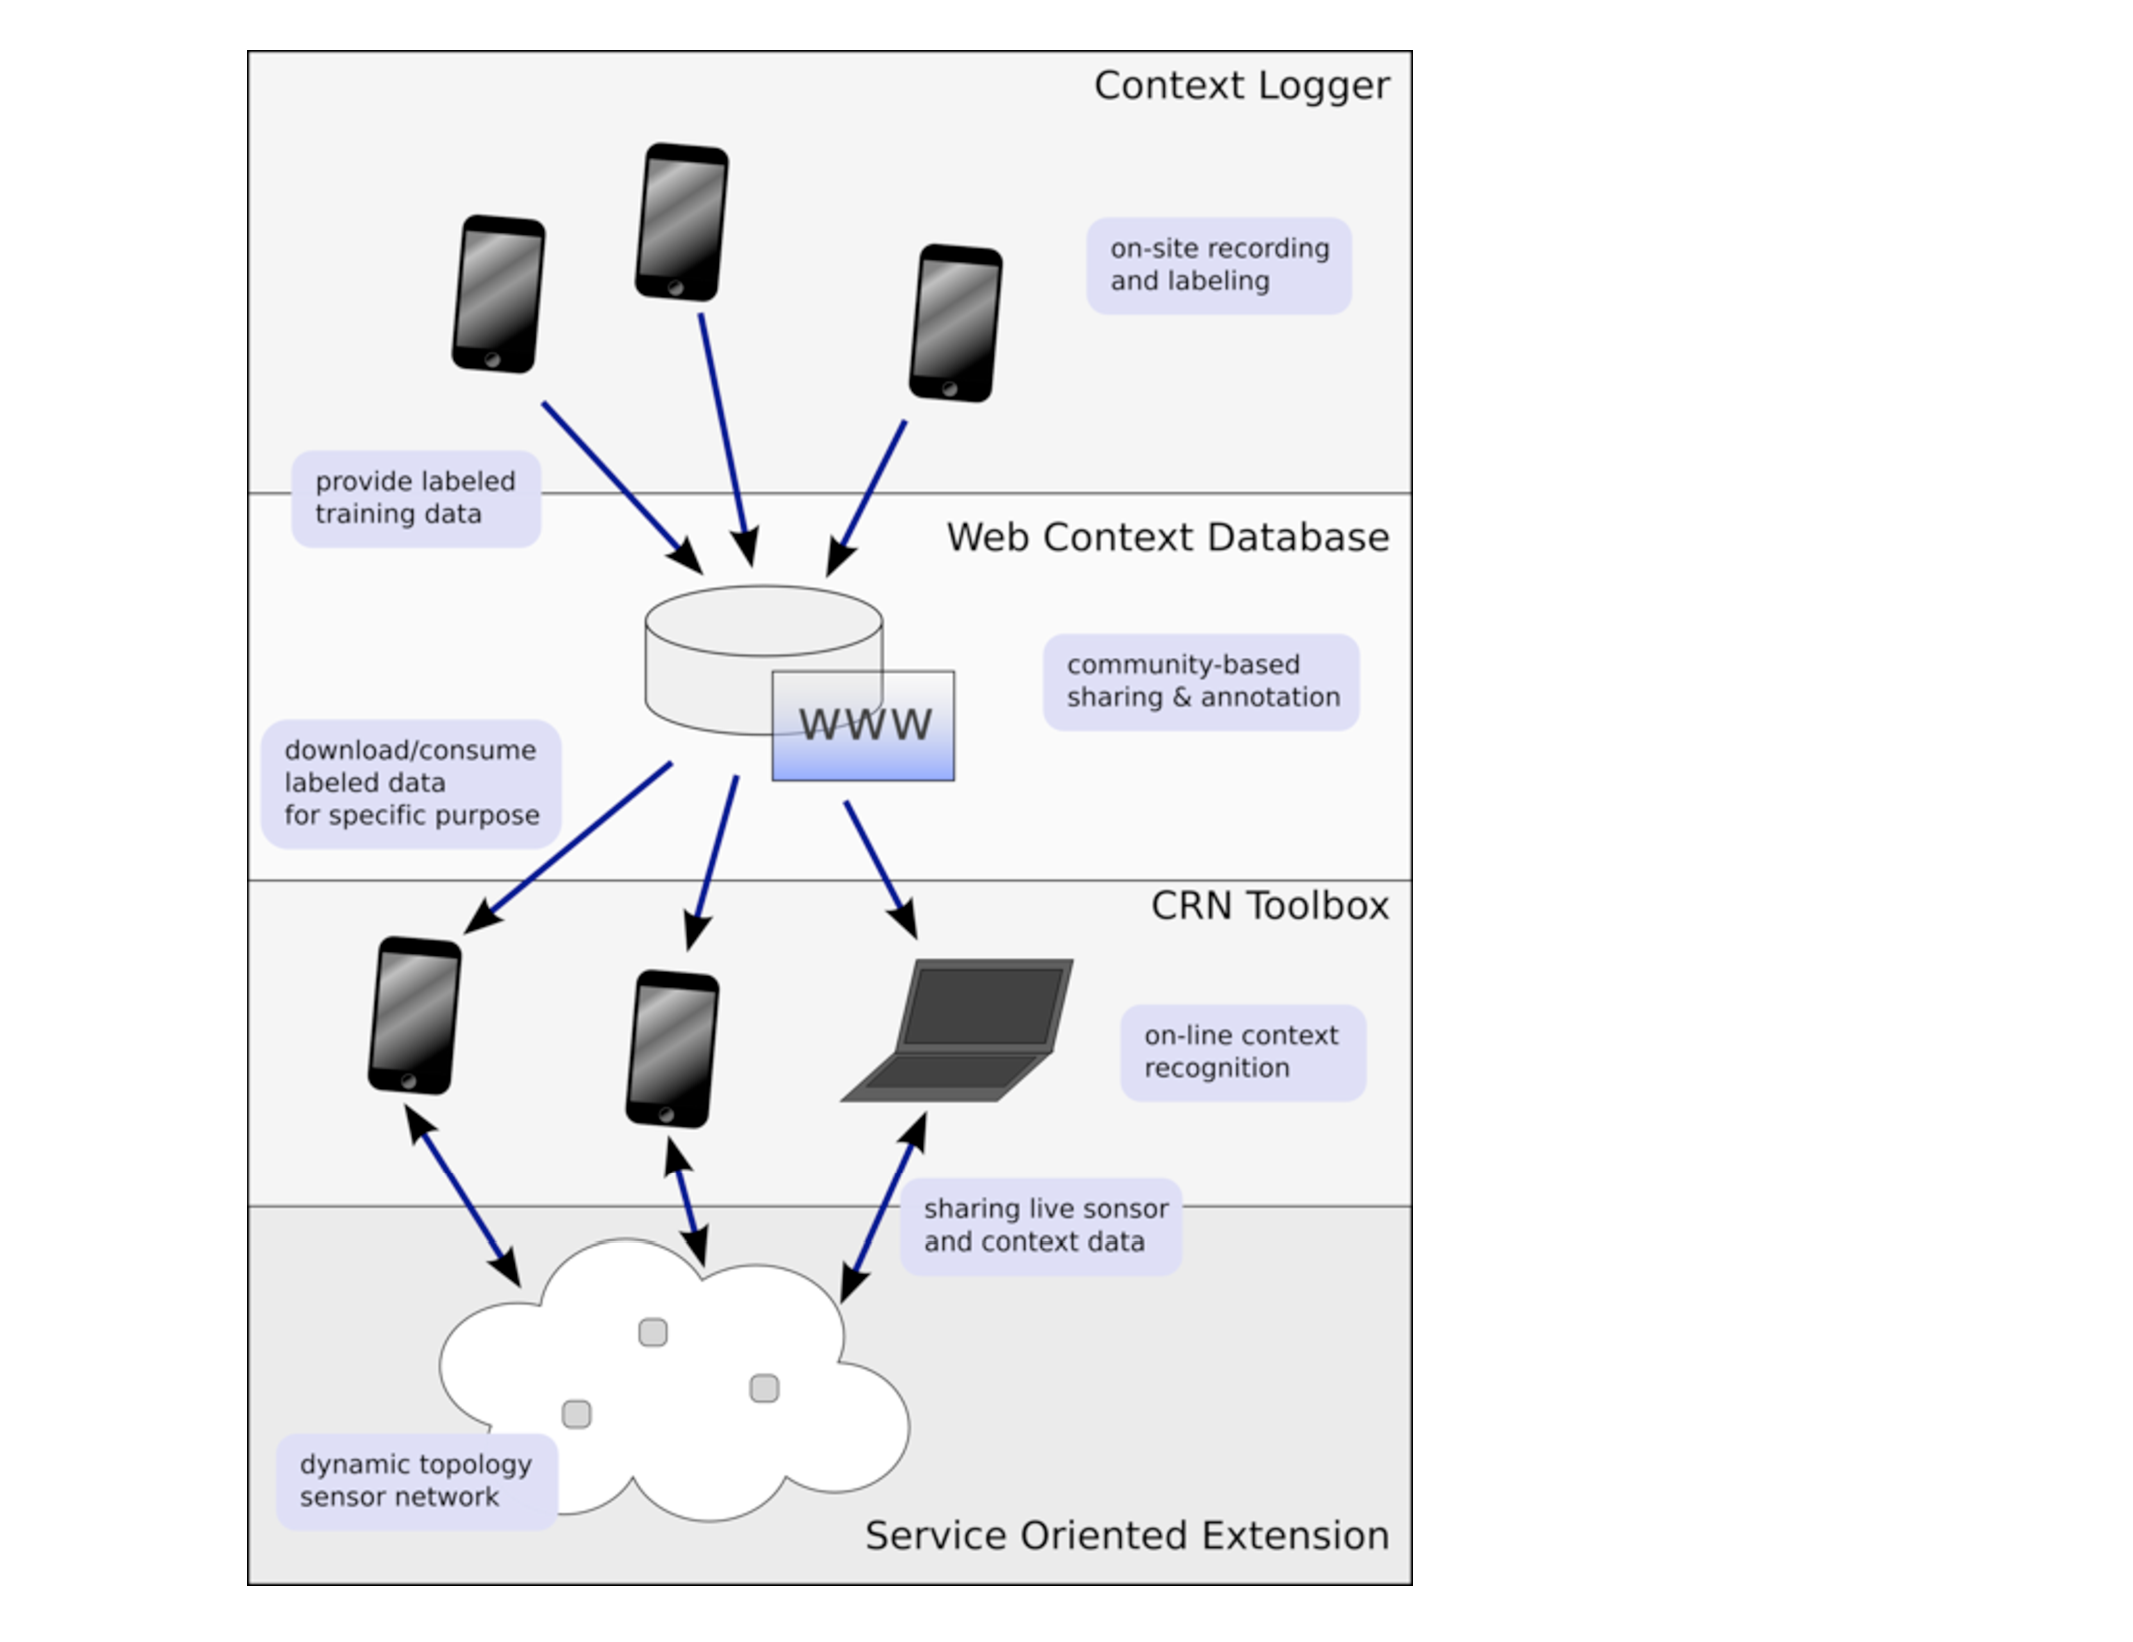
\includegraphics[height=3in]{bannach.pdf}
	\end{center}
  \caption[Activity sensing data collection]{Activity sensing data collection, storage and usage
   vision from Bannach
   et. al.~\cite{Bannach:2010wt}} \label{fig:dbannach} \end{figure}




As the experimental results in sections~3.5 and 4.5 indicate, the
recognition accuracy is directly related to what kinds of activities
were recorded and how representative the data set is towards the
anticipated application use cases. There is an
ongoing effort in the community to build a large, shared corpus of
standard context recognition data sets~(\cite{5573462}).
Similar datasets already exist for image or voice recognition.
Recording large scale context recognition datasets 
is a major effort due to the following reasons.
\begin{description}
\item{User/Environment Augmentation} -- One needs to be able to deploy
all the different sensing devices, depending on the application scenario
this might prove difficult. If a lot of onbody devices are involved,
the user might be hindered in the natural execution of the tasks one wants to record.
\item{Device Management} -- As the setup gets more and more complex,
it gets harder and harder to manage all devices. Especially if research
prototypes are used, it is difficult to ensure that all devices record
and supply useful data.
\item{Synchronization} -- Of course, the sensor streams also need to be
synchronized. Activity class assignments get especially tricky if
the sensing devices do not supply a steady sampling rate etc. 
\end{description}

Notable are the efforts and
achievements of Bannach to build rapid prototyping systems for
activity recognition and to enable easy monitoring, conduction and
sharing of context recognition
experiments~(\cite{Bannach:2010wt,Bannach:2008vl}). 

\subsection{Sensor Exchangeability and Abstraction}

\begin{figure}[t]
  \begin{center}
  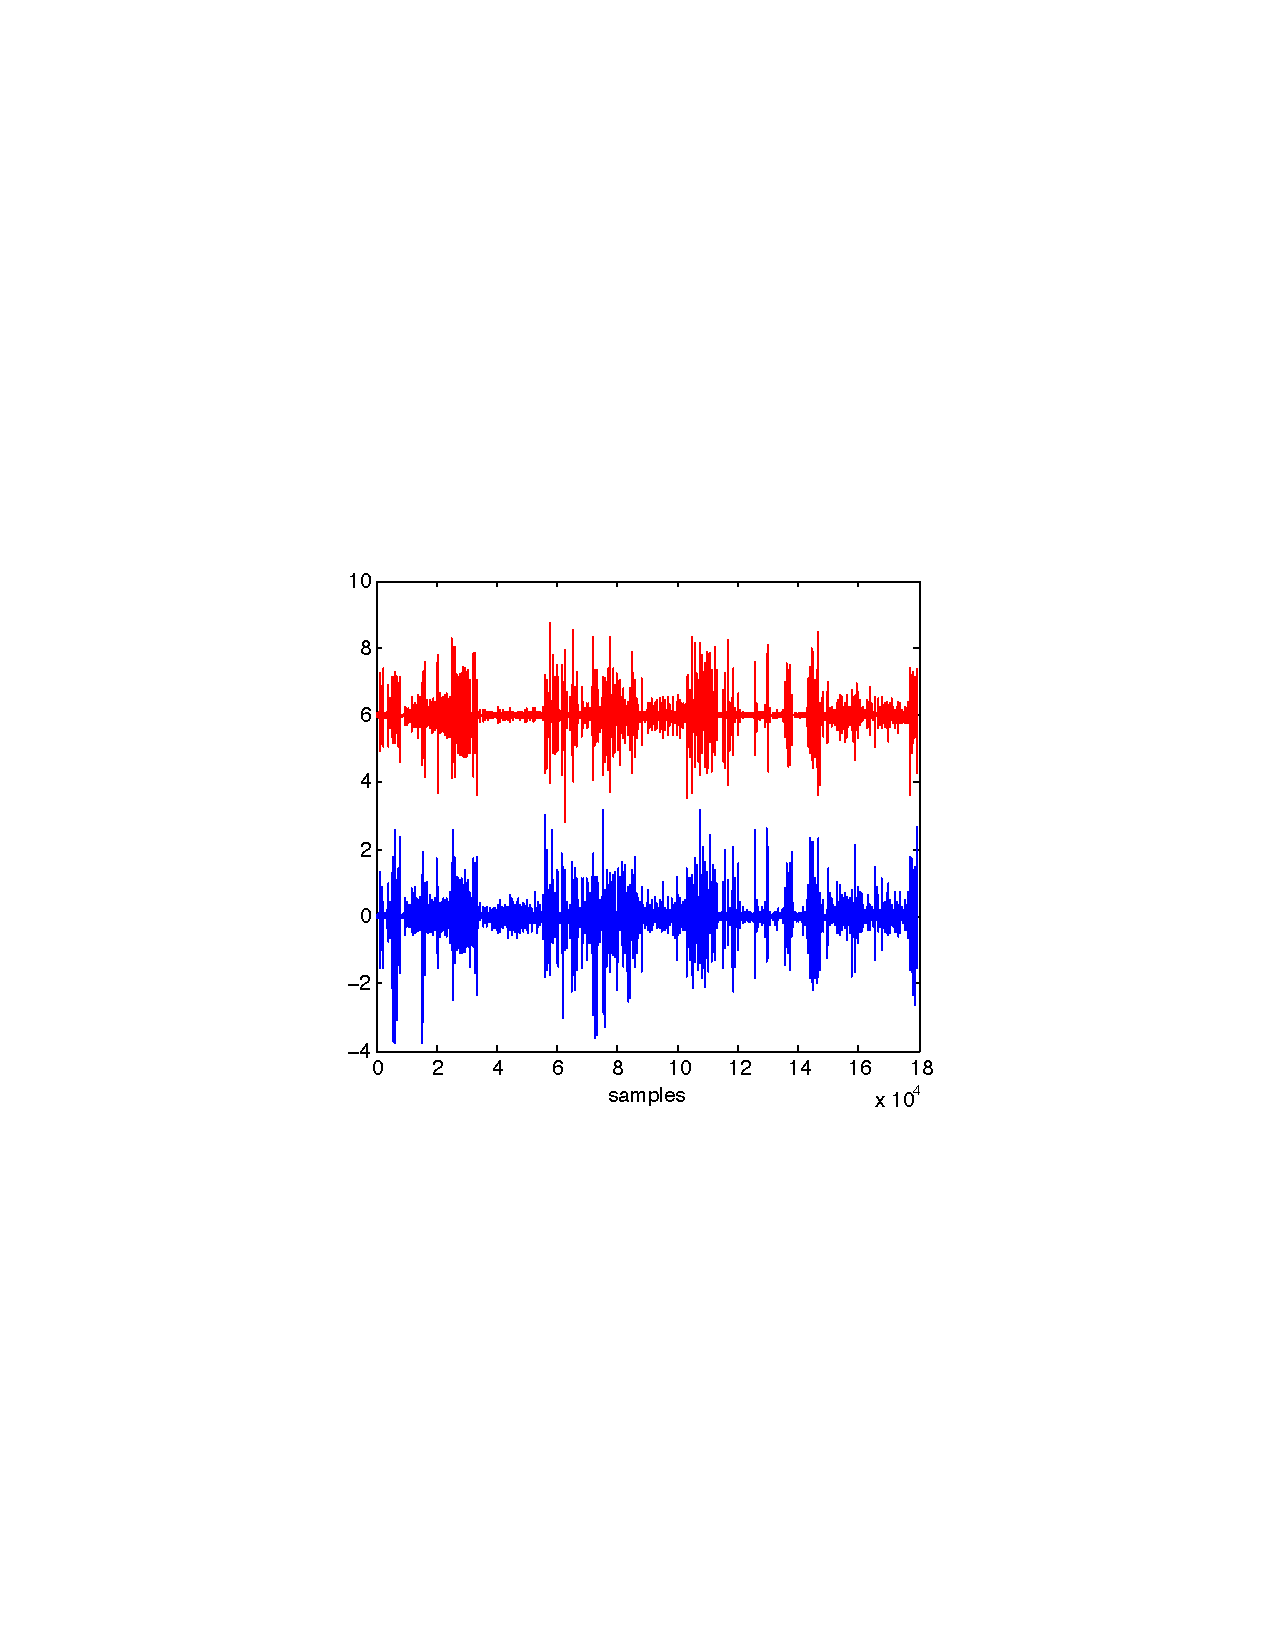
\includegraphics[height=3in]{maggyrosignal.pdf}
	\end{center}
  \caption[Estimated gyro signal]{Example traces of signal level estimation of angular
   velocity using the magnetic field sensor. The original gyro
   signal is on top with an offset of 6
   rad/s.} \label{fig:gyromag} \end{figure}

To make pervasive applications more robust to devices -and with them
sensor modalities- vanishing and appearing, the question "Are there
similar sensors that can replace each other to a certain degree?"
gains importance. Take the concept of location again, which is well
understood by research and partly adopted by industry. The iphone sdk
lets developers not select directly which method/sensor they want to
use (either cell-tower triangulation, wifi-maps or GPS). The modality
is chosen by the CoreLocation library depending on the developer's
needs. This encapsulation is highly appreciated for other types of
sensor modalities. Yet, beforehand we need to determine to what extend
similar sensors and inference methods can replace each other. 
As a first step, we already presented a detail study on to what extend
magnetic field sensors can replace gyroscopes
(\cite{Kunze:2010he,Bahle:2010ww}. This is in the same line of thought
as the work from Laerhoven, comparing ball switches to accelerometers.

Yet, for activity recognition to become a "invisible technology" using
Mark Weiser's term, we need higher level abstractions. As most activity
recognition is special purpose, application dependent, this task is not
trivial. Although a straight forward abstraction to introduce
includes human motion, e.g. 'a modes of locomotion sensor' that can
recognize walking, standing etc. If this inference is achieved
over a ball switch, gyro, accelerometer etc. should be handled transparently
(maybe only returning some performance characteristics, similar to
the location framework). Also a human can only move his arms a certain
way, e.g. lift sth., pull. Useful activities need to be classified
and combined in those virtual sensors.

This development is crucial for broad adoption of activity recognition.
As of today, you need experts to design and implement an activity recognition
system and to find the right sensors, features and classifiers for
the task at hand, especially for non-trivial activities, 
is sadly more an art than science. Yet, if we are able to create these
building blocks regular application developer can use them as they 
rely on the location frameworks today without caring about the
actual sensor hardware or the inference type.

More crucial and more important, a higher level activity description
allows for an easier deployment and better re-usability. So far,
activity recognition systems are more or less islands written for
a specific purpose, executed on predefined hardware. In my opinion,
this is a major reason for their limited adoption.

\subsection{Crowdsourcing}

One of the major problems in activity recognition is most algorithms
and systems need precise class labels assigned by an expert to work
correctly. This effect gets worse with large scale, crowd-based sensing
on phones, especially dealing with collective activities, 
as label to data assignment is more ambiguous.

However, most people regularly use microblogging services from their phones.
According to Twitter, a prominent microblogging site
with over 200 million users, 62 percent of their users
access the service over a mobile client\footnote{http://blog.twitter.com/2010/09/evolving-ecosystem.html}.
Unfortunately, as such the ground truth from twitter is noisy and
not easily interpretable (e.g. there are time delays between event and tweet).
As such we need to better understand the processes between the social activity flow the events
and its relation to the messages. 

We use soccer games as an example for the integration between crowed based sensing and
microblogging, due to two main reasons. First of all, a soccer game 
provides an objective, easily recognizable ground truth (e.g. a goal is shot, people are happy/sad)
compared to other large events. Second, compared to a concert etc., it contains very diverse events,
that in turn have a natural order and, thus, can be interpreted as an activity flow model. 
From users wearing smart phones at these events we gathered sensor data. 

\begin{figure}[t]
\centering{
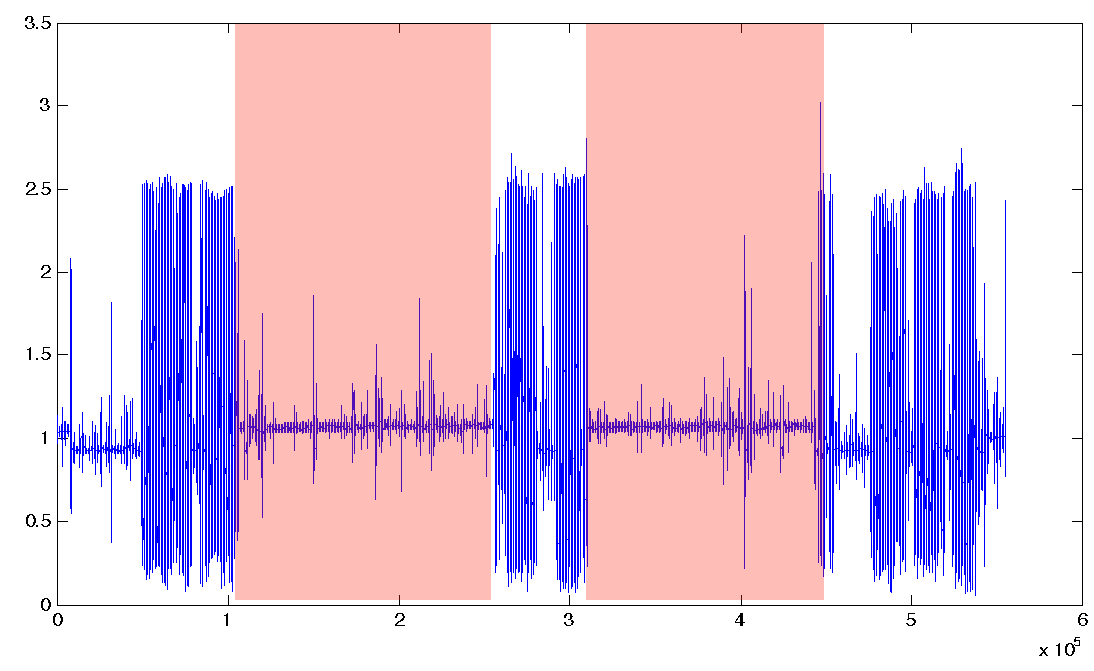
\includegraphics[scale=0.35]{accel.pdf}
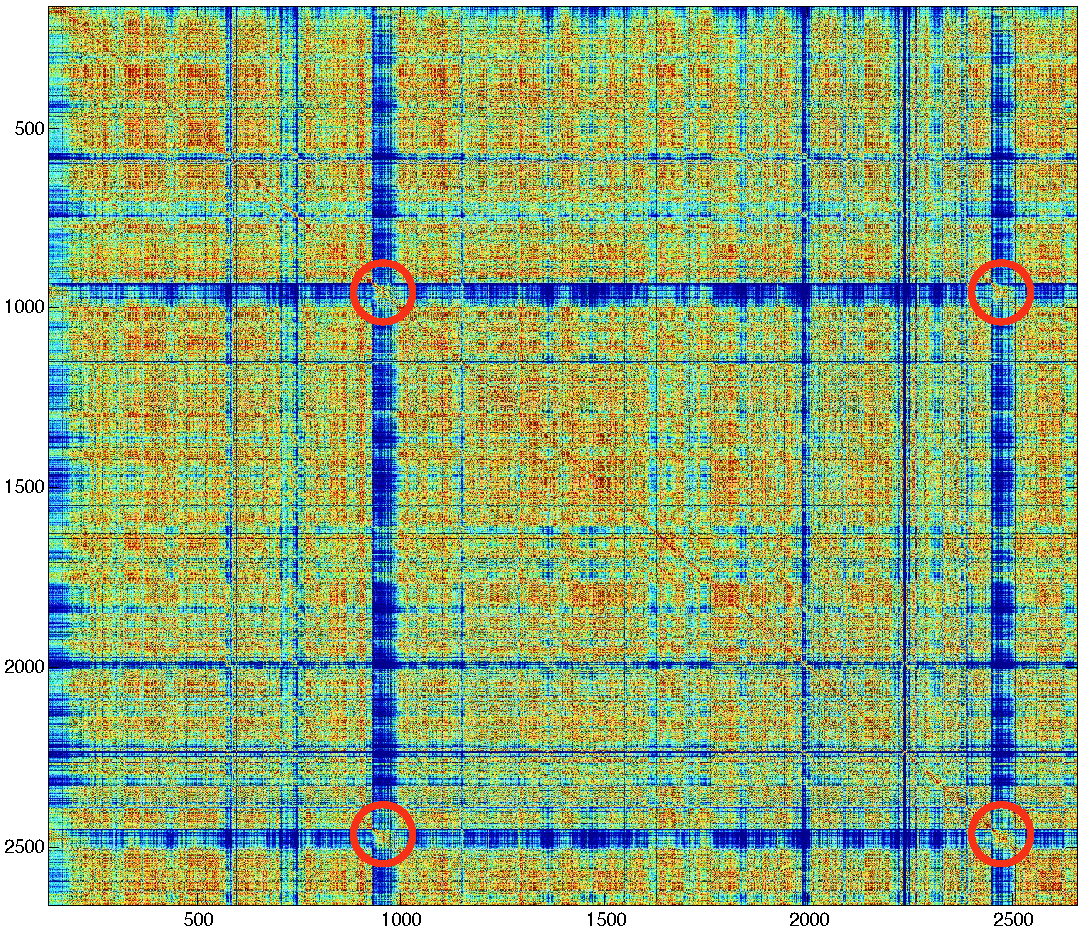
\includegraphics[scale=0.3]{correlation.pdf}
}
\caption[Soccer game sound and acceleration]{On the left: accelerometer norm from a mobile phone recorded from a fan during a soccer game. The two halfs of the game
can be easily recognized. Right: correlation matrix between audio features of two mobile phones during a soccer game. The places marked 
with red circles indicate 2 goals. }
\label{fig:acceleration}
\end{figure}

The structure and main events during the game are captured by combining data from different users.
Figure~\ref{fig:acceleration} depicts the acceleration norm from one user during a game. Start, stop and half time break 
can be easily seen. Combining several acceleration logs one can filter out specific events for a user
(e.g. getting sth. to drink), compared to "global" events (e.g. doing a Laola Wave). These global signal events, in turn, can
be concatenated to event flows. The same holds for sound. Figure~\ref{fig:acceleration} 
depicts a correlation between sound features of two phones from a soccer game. 
X and y axis are the feature samples over time. Of course, we see a high correlation in the diagonal. 
The two goals shot during this recording are clearly visible in plot (red circles). They correlate high with themselves, however low with the rest.

We believe the combination of microblogging information and
traditional activity recognition sensors aggregated over multiple users
is very valuable. 
There are 2 more use cases for microblogging we want to mention:
\begin{description}
 \item{"Novel sensor modality"}-
The straight forward way to deal with status updates
in Twitter, Facebook and other microblogging services is to use them as another
input for the inferencing algorithms. In the last year, there have been a couple of 
papers showing the merits of this, especially in the aftermath of a disaster(\cite{Vieweg:2010jd}). However,
to our knowledge, so far nobody combined the inferences derived from microblogging messages with
conventional context recognition sensor data.
 \item{User modeling} - Twitter and other microblogging services offer a history about
the user. One can extract information like age group, education and special interests
from the user by mining his history and incorporating the users he follows. This has been
already done in the natural language community, yet is not yet applied to ubicomp 
applications.
\end{description}

%\begin{figure}[t]

%\centering  
%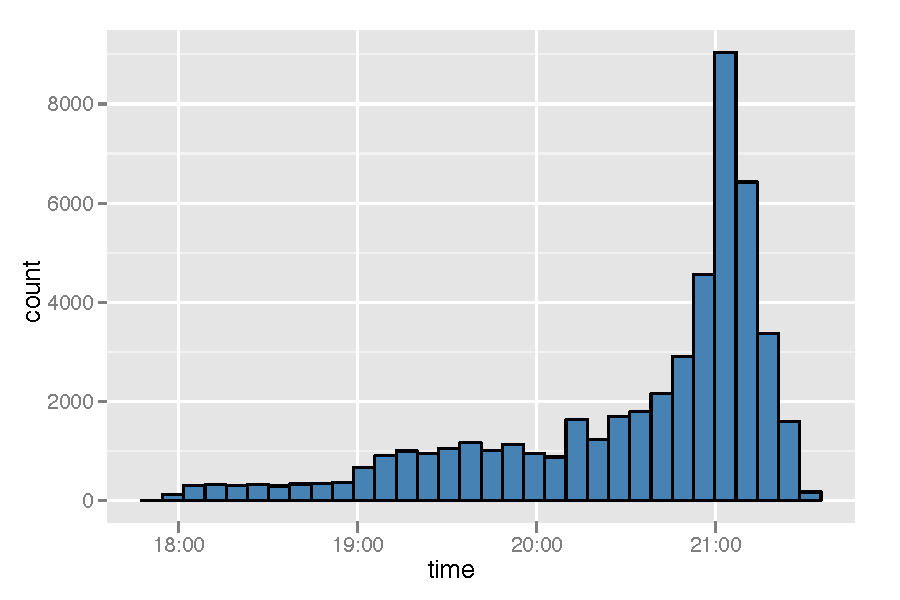
\includegraphics[scale=0.43]{all.pdf}
%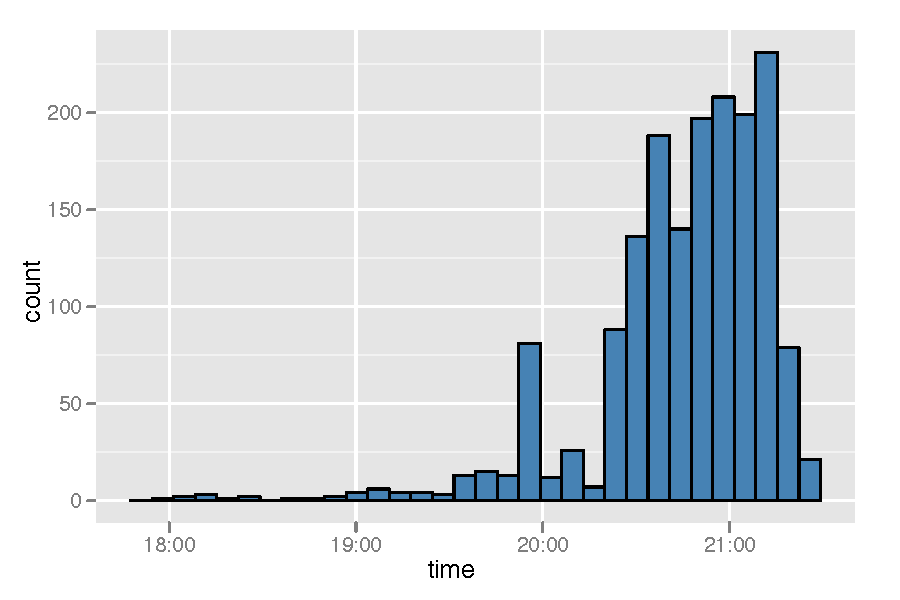
\includegraphics[scale=0.43]{goal.pdf}
%\caption{Histogram of recorded twitter messages during French/England friendship game. On the left, the histogram
%of all messages that contain the specific keywords, on the left, only the messages containing "goal".}
%\label{fig:twitter}

%\end{figure}
%We recorded twitter data containing keywords from the soccer match, England vs. France, on 10.11.2010. 
%We so far processed the tweets from the first half time and only the first part of the second.
%England lost 2:1 with goals for France at 20:20 and 21:19. 
%From the frequency of all recorded twitter messages we can detect that most people seem to tweet just at the beginning
%of the second half. Just looking at the frequency of the word goal in these twitter messages, we see a spike just
%before the start of the game. These are mainly wishes (e.g. "I hope England scores a lot of goals").
%Then 16 min in the game (kickoff 20:04), the people celebrate the first French goal. However, the second goal cannot
%be that easily seen. There is a spike at 21:19, yet after the first goal, the frequency of the word did not really die down.

%\begin{figure}[t]
%\centering  
%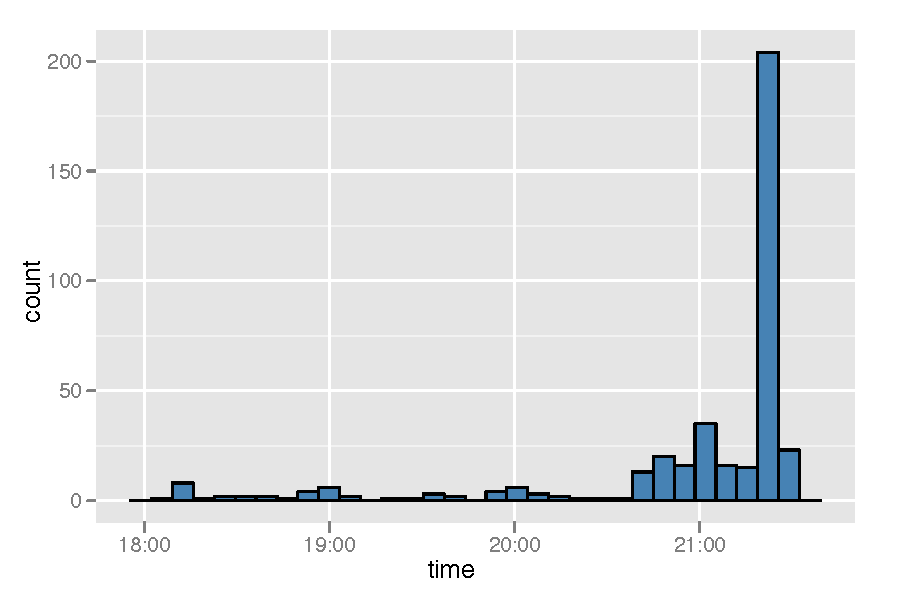
\includegraphics[scale=0.55]{player.pdf}
%\caption[Twitter histogram]{Histogram of recorded twitter messages during French/England friendship game only the messages containing "Valbuena", a player
%scoring the second goal at 21:19.}
%\label{fig:twitter2}
%
%\end{figure}
%Taking the frequency of "Valbuena", the name of the french player shooting the second goal,
%we get the goal event in a 4 min. window, as depicted in Figure~\ref{fig:twitter2}. 
%Just using this string matching approach, several applications are can
%already be envisioned, from a simple access and capture system associating the most frequently used player name
%with the game recordings to a system that directly comments the game live or gives best-of-scenes to a user
%inferring his team, player and game situation preferences.
%
%From the case study we can extrapolate that microblogging enhances context recognition systems. Yet to fully use
%its potential there are several challenges that need to be tackled. We list some of them below.
%\vspace{-2pt}
%\begin{description}
%\item{Dealing with Noise}-Using the raw twitter real-time stream can be overwhelming. In the soccer game example
%we used keywords associated with the specific event. We still gathered a fair amount of unwanted noise. A substantial amount
%of tweets (in our case 35 \%) also contains the location of the user, giving additional means of filtering.
% \item{Modeling of the ripple effects}-
%The game data indicates that it is possible to use twitter messages even as "real time" sensing modality, at least for 
%the most important events in soccer games (goals). Yet, the ripple effects and time delays in messages is something
%that needs to be better understood. People tend to tweet a specific event when it happens, 
%yet also with some delay to when they have time. Therefore, we see an increase 
%in twitter messages during and just after the half time break.
%\item{Natural Language Processing and Fusion Algorithms}- 
%Instead simple keyword search, some tailored inference is needed. Sensible fusion algorithms and the relationship
%between microblogging and other sensors needs to be investigated.
%\end{description}

\bibliographystyle{abbrv} \bibliography{conclusion}
